% Subsection of App. "External Evaluation in Detail": LCS on ASAP 2.0 persuasive essays
% (summarized in Sec. 3.2, "Evaluation on Natural Text").
% Every number is a macro generated by scripts/asap_lcs.py (asap_numbers.tex); the figure by
%   uv run --with matplotlib python scripts/asap_lcs.py --tag 120 figure --out figures/fig_asap.pdf

%% ----------------------------------------------------------------------------
\subsection{Essay Quality: ASAP~2.0 Persuasive Essays}
\label{app:asap}

Does the score track how good an argument is when nothing about the text was built for it? We
read $\LCS$ on student essays that trained raters scored for overall quality, with the full
pipeline running end to end: claims are extracted, relations are mined, and truth values come
from checking each claim against the article the students wrote about. The setting lies outside
the one the score's guarantee covers. Every essay has its own claims, so essays are compared on
the score's common scale, not by the coherence order. The question is correlational: is $\LCS$
higher for essays the raters scored higher, and does it tell us anything that essay length does
not?

\paragraph{Data.} ASAP~2.0 \citep{crossley2025asap} has source-based persuasive essays by students
in grades 6--10, each scored holistically from 1 (little mastery) to 6 (clear and consistent
mastery) on a rubric that covers critical thinking, the use of evidence from the source,
organization and language. We use one prompt, so that every essay argues from the same article:
students read ``Making Mona Lisa Smile'', on software that recognizes emotions from facial
movements (the Facial Action Coding System), and argue whether using it to read students'
emotions in class is valuable. We drew \asapPerLevel{} essays per score level, \asapEssays{} in
all, from the released training and test files, stratified within each level by length quartile
so that each level keeps its natural spread of lengths. The essays have \asapWordsMin--\asapWordsMax{}
words. The 18 essays of an earlier pilot are excluded.

\paragraph{Pipeline.}
\begin{itemize}[leftmargin=1.2em,itemsep=1pt,topsep=2pt]
\item \textbf{Claims.} The FactReasoner atomizer (GPT-6) splits each essay into
  \asapClaimsMin--\asapClaimsMax{} claims (median \asapClaimsMedian; \asapClaims{} in all). We add
  one rule to its prompt for essays: state the writer's own claims and opinions directly, never as
  ``the author states\,\ldots''. Without the rule the atomizer turns the student's opinions into
  claims about an unnamed ``author'', which readers and the source check take to mean the
  article's author.
\item \textbf{Relations.} The graph-level miner (GPT-6, $K{=}5$, the taxonomy of
  Table~\ref{tab:couplings}) finds \asapRelations{} relations, \asapRelationsMean{} per essay:
  \asapSenseEvidence\% \sense{Evidence}, \asapSenseCauseEffect\% \sense{Cause-Effect} and
  \asapSenseRestatement\% \sense{Restatement}, with almost no \sense{Refutation}. $\Lambda$ is
  computed exactly by variable elimination on each connected component (the largest has
  \asapLargestComp{} claims; induced width at most \asapMaxWidth), with flat priors.
\item \textbf{Truth values.} Each claim is checked against a transcription of the article by a
  three-vendor committee (GPT-6.1, Gemini~3.1 Pro, Claude Opus~5.5, majority of three), using
  no outside knowledge. The majority labels are: \asapLabOpinion{} opinions or reasoning,
  \asapLabSupported{} supported, \asapLabNotinsource{} factual but not in the article,
  \asapLabContradicted{} contradicted, and \asapLabUnresolved{} without a majority. The three
  models agree on \asapUnanimous\% of claims.
\end{itemize}

\paragraph{Committed worlds.} An essay's opinions and reasoning cannot be checked against the
article, so they keep their asserted value in every world. Setting them to $0$ would turn every
reason the student gives for an opinion into a conflict. We read $\LCS$ at three worlds:
\begin{itemize}[leftmargin=1.2em,itemsep=1pt,topsep=2pt]
\item \emph{asserted}: every claim true, the internal-coherence reading;
\item \emph{source}: a claim is false when the article contradicts it;
\item \emph{strict}: a claim is also false when it is factual but not in the article, the binary
  verdict convention of \S\ref{sec:setup} applied to factual claims only.
\end{itemize}

\begin{table*}[t]
\centering\small
\setlength{\tabcolsep}{6pt}
\begin{tabular}{@{}lccc@{}}
\toprule
& $\rho$ & partial, length & partial, length + judge \\
\midrule
words & \asapRhoWords\asapCI{\asapRhoWordsLo}{\asapRhoWordsHi} & -- & -- \\
claims & \asapRhoClaims\asapCI{\asapRhoClaimsLo}{\asapRhoClaimsHi} & \asapParClaims\asapCI{\asapParClaimsLo}{\asapParClaimsHi} & \\
relations & \asapRhoRelations\asapCI{\asapRhoRelationsLo}{\asapRhoRelationsHi} & \asapParRelations\asapCI{\asapParRelationsLo}{\asapParRelationsHi} & \asapPwjRelations\asapCI{\asapPwjRelationsLo}{\asapPwjRelationsHi} \\
\midrule
$\LCS$, asserted & \asapRhoLcsAsserted\asapCI{\asapRhoLcsAssertedLo}{\asapRhoLcsAssertedHi} & \asapParLcsAsserted\asapCI{\asapParLcsAssertedLo}{\asapParLcsAssertedHi} & \asapPwjLcsAsserted\asapCI{\asapPwjLcsAssertedLo}{\asapPwjLcsAssertedHi} \\
$\LCS$, source & \asapRhoLcsSource\asapCI{\asapRhoLcsSourceLo}{\asapRhoLcsSourceHi} & \asapParLcsSource\asapCI{\asapParLcsSourceLo}{\asapParLcsSourceHi} & \asapPwjLcsSource\asapCI{\asapPwjLcsSourceLo}{\asapPwjLcsSourceHi} \\
$\LCS$, strict & \asapRhoLcsStrict\asapCI{\asapRhoLcsStrictLo}{\asapRhoLcsStrictHi} & \asapParLcsStrict\asapCI{\asapParLcsStrictLo}{\asapParLcsStrictHi} & \asapPwjLcsStrict\asapCI{\asapPwjLcsStrictLo}{\asapPwjLcsStrictHi} \\
$\Lambda$ per claim, asserted & \asapRhoLpcAsserted\asapCI{\asapRhoLpcAssertedLo}{\asapRhoLpcAssertedHi} & \asapParLpcAsserted\asapCI{\asapParLpcAssertedLo}{\asapParLpcAssertedHi} & \\
conflicts, asserted & \asapRhoConflictsAsserted\asapCI{\asapRhoConflictsAssertedLo}{\asapRhoConflictsAssertedHi} & \asapParConflictsAsserted\asapCI{\asapParConflictsAssertedLo}{\asapParConflictsAssertedHi} & \\
conflicts, strict & \asapRhoConflictsStrict\asapCI{\asapRhoConflictsStrictLo}{\asapRhoConflictsStrictHi} & \asapParConflictsStrict\asapCI{\asapParConflictsStrictLo}{\asapParConflictsStrictHi} & \\
\midrule
DiscoScore RC & \asapRhoDiscourseRc\asapCI{\asapRhoDiscourseRcLo}{\asapRhoDiscourseRcHi} & \asapParDiscourseRc\asapCI{\asapParDiscourseRcLo}{\asapParDiscourseRcHi} & \\
DiscoScore LC & \asapRhoDiscourseLc\asapCI{\asapRhoDiscourseLcLo}{\asapRhoDiscourseLcHi} & \asapParDiscourseLc\asapCI{\asapParDiscourseLcLo}{\asapParDiscourseLcHi} & \\
entity graph & \asapRhoDiscourseEntityGraph\asapCI{\asapRhoDiscourseEntityGraphLo}{\asapRhoDiscourseEntityGraphHi} & \asapParDiscourseEntityGraph\asapCI{\asapParDiscourseEntityGraphLo}{\asapParDiscourseEntityGraphHi} & \\
G-Eval, GPT-6 & \asapRhoJudgeGevalGptSixSol\asapCI{\asapRhoJudgeGevalGptSixSolLo}{\asapRhoJudgeGevalGptSixSolHi} & \asapParJudgeGevalGptSixSol\asapCI{\asapParJudgeGevalGptSixSolLo}{\asapParJudgeGevalGptSixSolHi} & \\
\bottomrule
\end{tabular}
\caption{\textbf{Agreement with the human essay scores} (\asapEssays{} essays, \asapPerLevel{} per
score level). Spearman $\rho$ with the score; then the partial Spearman correlation with the
ranks of word count removed, and with both word count and the G-Eval coherence judge (mean of
five runs) removed. Brackets: 95\% percentile bootstrap intervals, resampling essays within score
level (2{,}000 resamples).}
\label{tab:asap-corr}
\end{table*}

\begin{table}[t]
\centering\footnotesize
\setlength{\tabcolsep}{2.6pt}
\begin{tabular}{@{}lcccccc@{}}
\toprule
score & 1 & 2 & 3 & 4 & 5 & 6 \\
\midrule
words & \asapLvlOneWords & \asapLvlTwoWords & \asapLvlThreeWords & \asapLvlFourWords & \asapLvlFiveWords & \asapLvlSixWords \\
claims & \asapLvlOneClaims & \asapLvlTwoClaims & \asapLvlThreeClaims & \asapLvlFourClaims & \asapLvlFiveClaims & \asapLvlSixClaims \\
relations (mean) & \asapLvlOneRels & \asapLvlTwoRels & \asapLvlThreeRels & \asapLvlFourRels & \asapLvlFiveRels & \asapLvlSixRels \\
$\LCS$, asserted & \asapLvlOneLcsAsserted & \asapLvlTwoLcsAsserted & \asapLvlThreeLcsAsserted & \asapLvlFourLcsAsserted & \asapLvlFiveLcsAsserted & \asapLvlSixLcsAsserted \\
$\LCS$, strict & \asapLvlOneLcsStrict & \asapLvlTwoLcsStrict & \asapLvlThreeLcsStrict & \asapLvlFourLcsStrict & \asapLvlFiveLcsStrict & \asapLvlSixLcsStrict \\
conflicts, strict (mean) & \asapLvlOneConfStrict & \asapLvlTwoConfStrict & \asapLvlThreeConfStrict & \asapLvlFourConfStrict & \asapLvlFiveConfStrict & \asapLvlSixConfStrict \\
not in the article & \asapLvlOneNis & \asapLvlTwoNis & \asapLvlThreeNis & \asapLvlFourNis & \asapLvlFiveNis & \asapLvlSixNis \\
\bottomrule
\end{tabular}
\caption{\textbf{By score level.} Medians, except where marked as means; ``not in the article''
is the mean share of an essay's claims that are factual but absent from the article.}
\label{tab:asap-levels}
\end{table}

\begin{figure*}[t]
\centering
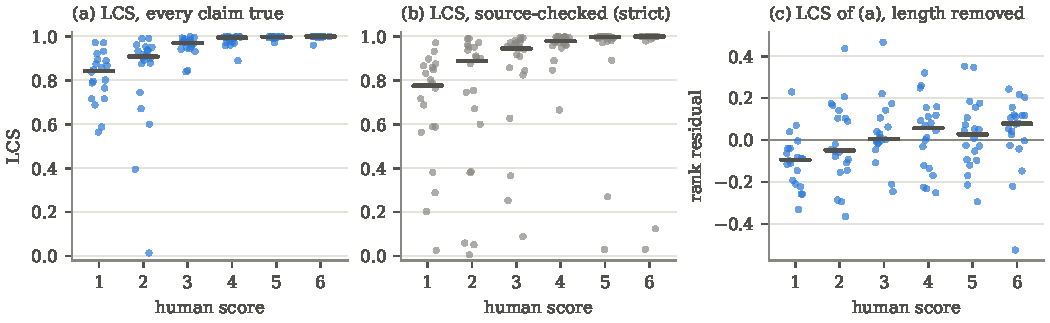
\includegraphics[width=\textwidth]{figures/fig_asap.pdf}
\caption{\textbf{$\LCS$ against the human essay score}, one dot per essay and a bar at each
level's median. (a) Every claim true. (b) The strict source-checked world: claims that are
factual but not in the article are false. (c) The score of (a) with length removed: the residual
of its rank after regressing on the rank of the word count, as a share of the sample, which is
what the partial correlation of Table~\ref{tab:asap-corr} measures.}
\label{fig:asap}
\end{figure*}

\paragraph{Why length matters.} Length is the classic confound of essay scoring. Stronger students
write more, and the rubric rewards developed arguments, which take words, so word count alone
correlates with the score at \asapRhoWords. $\LCS$ grows with length too, for mechanical reasons:
\begin{itemize}[leftmargin=1.2em,itemsep=1pt,topsep=2pt]
\item a longer essay has more claims (their number correlates with the score at
  \asapRhoClaims), so the miner has more pairs to link and finds more relations;
\item with every claim true, every relation it finds is a support unless it is a conflict, and
  conflicts are rare (\asapConfAsserted{} in all \asapEssays{} essays);
\item each support adds a positive term to $\Lambda$ (Lemma~\ref{lem:edit}), so more relations push
  $\Lambda$, and with it $\LCS$, upwards.
\end{itemize}
A long but mediocre essay can therefore outscore a short, tight one simply because it contains more
linked claims, and a raw correlation between $\LCS$ and the score cannot tell whether $\LCS$ tracks
quality or only the amount of text. We ask a narrower question instead: among essays of similar
length, do the higher-scored ones have higher $\LCS$?

\paragraph{Removing length: partial rank correlation.} Let $r(\cdot)$ map a variable to its ranks
over the $n=\asapEssays$ essays, with ties given their average rank. For a metric $m$ (here $\LCS$),
the human score $s$ and the word count $w$, we fit $r(m)$ and $r(s)$ separately by least squares on
$r(w)$ and an intercept, and keep the residuals
\[
  e_x = r(x) - \bigl(\hat a_x + \hat b_x\, r(w)\bigr), \qquad x\in\{m,s\},
\]
the part of each ranking that a linear function of the length ranking does not explain. The
partial correlation after length is the Pearson correlation of the two residuals,
$\rho_{ms\cdot w}=\operatorname{corr}(e_m,e_s)$: it is positive when, at a given length, the
essays ranked higher by $m$ are also ranked higher by the raters. To remove the G-Eval judge as
well, the regression has two predictors, $r(w)$ and the rank of the judge's score. Panel (c) of
Figure~\ref{fig:asap} plots $e_m$, as a share of $n$, against the score. The 95\% intervals are
percentile bootstraps over 2{,}000 resamples of essays, drawn with replacement within each score
level so that every resample keeps \asapPerLevel{} essays per level; each resample recomputes the
ranks, the regressions and the correlation. Two features of the method bear on how to read the
result:
\begin{itemize}[leftmargin=1.2em,itemsep=1pt,topsep=2pt]
\item \textbf{It is conservative.} Part of why good essays are long is that they argue more, so
  removing length also removes some genuine quality signal.
\item \textbf{It removes only the rank-linear part of the length effect.} A dependence on length
  that is not linear in rank, or that interacts with the score, can survive it. The nonlinear
  controls below relax this; the within-tertile correlations are a weaker check, since length still
  varies within each third.
\end{itemize}

\paragraph{Robustness.} Nonlinear length controls give the same picture: a cubic in the length
rank leaves \asapRobCubic{} \asapCI{\asapRobCubicLo}{\asapRobCubicHi}, and 6, 10 and 20 equal-count
length bins leave \asapRobBinsSix, \asapRobBinsOneZero{} and \asapRobBinsTwoZero. A count of
argumentative connectives (\emph{because}, \emph{therefore}, \emph{for example} and 19 others)
correlates with the score at \asapRhoConnectives{} but carries nothing beyond length
(\asapParConnectives), and $\LCS$ keeps \asapRobWordsConnectives{} once length and connectives are
both removed. Removing the number of mined relations as well leaves \asapRobWordsRelations{}
\asapCI{\asapRobWordsRelationsLo}{\asapRobWordsRelationsHi}, so $\LCS$ is more than a relation
count. The signed weight sum over the same graphs gives \asapParWsumAsserted{} after length. The
difference between the partial correlations of $\LCS$ and of G-Eval is \asapRobDiffGeval{}
\asapCI{\asapRobDiffGevalLo}{\asapRobDiffGevalHi}, so the two cannot be told apart here. A
grader prompted with the six-point holistic rubric (GPT-6, three runs averaged) correlates with the
score at \asapRhoJudgeRubricGptSixSol{} and at \asapParJudgeRubricGptSixSol{} after length, more than
$\LCS$; with length and the grader both removed, $\LCS$ keeps \asapPwrLcsAsserted{}
\asapCI{\asapPwrLcsAssertedLo}{\asapPwrLcsAssertedHi}, the signed sum \asapPwrWsumAsserted{} and
the relation count \asapPwrRelations, so the score carries information that a rubric grader
does not. Sampling
\asapPerLevel{} essays per level weights the extreme scores more than the natural score
distribution does, which inflates every correlation in the table.

\paragraph{Findings.} Table~\ref{tab:asap-corr} gives the correlations, Table~\ref{tab:asap-levels}
the levels and Figure~\ref{fig:asap} the essays.
\begin{itemize}[leftmargin=1.2em,itemsep=1pt,topsep=2pt]
\item \textbf{Most of the association runs through length.} With every claim true, $\LCS$ rises
  with the score ($\rho=\asapRhoLcsAsserted$), but word count alone does slightly better
  ($\asapRhoWords$). Once length is removed, $\asapParLcsAsserted$ remains, and $\asapPwjLcsAsserted$ remains once the
  G-Eval judge is removed as well. Within thirds of the length range, $\LCS$ still orders essays
  by score ($\asapTertShortRhoLcsAsserted$, $\asapTertMediumRhoLcsAsserted$,
  $\asapTertLongRhoLcsAsserted$ for short, medium and long essays), but so does word count
  ($\asapTertShortRhoWords$, $\asapTertMediumRhoWords$, $\asapTertLongRhoWords$), better in two of the
  three, so this check is weak. Removing length means
  removing much of what the raters reward, so the partial correlations are conservative. The
  number of claims carries nothing beyond length ($\asapParClaims$).
\item \textbf{The signal is support density, not conflict.} The count of mined relations carries
  most of the same signal ($\asapParRelations$ after length), and so does $\Lambda$ per claim
  ($\asapParLpcAsserted$). Conflicts carry none: with every claim true the miner finds
  \asapConfAsserted{} conflicts in all \asapEssays{} essays, in \asapConfEssaysAsserted{} of
  them. Students rarely contradict themselves. What separates a weak essay from a strong one is
  how many of its claims it ties together with reasons and evidence. $\LCS$ treats an unsupported
  claim as neutral, so a weak essay scores lower only because it earns fewer supports, never
  because it is penalized.
\item \textbf{Checking claims against the article does not help.} Contradicting the article is
  rare (\asapLabContradicted{} of \asapClaims{} claims), and the source world changes the
  correlations little ($\asapParLcsSource$ after length). The strict world lowers them
  ($\asapParLcsStrict$). Its conflicts, from reasoning to or from claims that are not in the
  article, occur at every score level (Table~\ref{tab:asap-levels}), so they add noise to the
  ordering rather than signal. An earlier pilot of \asapPilotN{} essays had suggested the
  opposite: after length, the strict world correlated at $\asapPilotParStrict$, against
  $\asapPilotParAsserted$ with every claim true. The atomizer rule, added after that pilot, does
  not explain the difference, since with it the two are $\asapPilotFixParStrict$ and
  $\asapPilotFixParAsserted$. With \asapPilotN{} essays the intervals are wide (the strict world
  with the rule gives
  $\asapPilotFixParStrict$\asapCI{\asapPilotFixParStrictLo}{\asapPilotFixParStrictHi}) and
  overlap those of Table~\ref{tab:asap-corr}; the pilot's ordering of the two worlds did not
  replicate.
\item \textbf{The score saturates on good essays.} From level 4 up the median $\LCS$ is at least
  $0.99$, and the ordering there rests on small differences. $\Lambda$, which does not saturate,
  gives the same correlations to two decimals; the essays have different claim sets, so this is
  an empirical agreement rather than a consequence of the map between the two.
\item \textbf{Baselines.} The G-Eval coherence judge (GPT-6) agrees with the raters less overall
  ($\asapRhoJudgeGevalGptSixSol$) and about as much once length is removed
  ($\asapParJudgeGevalGptSixSol$). The discourse-coherence baselines are weaker on both counts.
\end{itemize}

\paragraph{What this shows, and what it does not.} On natural essays, with claims and relations
mined and nothing built for the score, $\LCS$ agrees with human quality judgments beyond what
length and an LLM judge capture. It does so through the density of supported reasoning, which
is one of the things the rubric rewards. It is not a measure of essay quality. The holistic score
also rewards language, organization and the use of the source, which $\LCS$ does not see, and the
conflicts that drive $\LCS$ in the ladder benchmark are nearly absent from these essays.

The evidence has clear limits:
\begin{itemize}[leftmargin=1.2em,itemsep=1pt,topsep=2pt]
\item one prompt, one miner and one atomizer, with an essay-specific atomizer rule;
\item truth values from a model committee, not from people;
\item correlations that are rank-linear, with length controlled only through its rank;
\item a design that the pilot informed, although the pilot essays are not in the sample.
\end{itemize}
